% CS 111 style
% Typical usage (all UPPERCASE items are optional):
%       \input 111pre
%       \begin{document}
%       \MYTITLE{Title of document, e.g., Lab 1\\Due ...}
%       \MYHEADERS{short title}{other running head, e.g., due date}
%       \PURPOSE{Description of purpose}
%       \SUMMARY{Very short overview of assignment}
%       \DETAILS{Detailed description}
%         \SUBHEAD{if needed} ...
%         \SUBHEAD{if needed} ...
%          ...
%       \HANDIN{What to hand in and how}
%       \begin{checklist}
%       \item ...
%       \end{checklist}
% There is no need to include a "\documentstyle."
% However, there should be an "\end{document}."
%
%===========================================================
\documentclass[11pt,twoside,titlepage]{article}
%%NEED TO ADD epsf!!
\usepackage{threeparttop}
\usepackage{graphicx}
\usepackage{latexsym}
\usepackage{color}
\usepackage{listings}
\usepackage{fancyvrb}
%\usepackage{pgf,pgfarrows,pgfnodes,pgfautomata,pgfheaps,pgfshade}
\usepackage{tikz}
\usepackage[normalem]{ulem}
\tikzset{
    %Define standard arrow tip
%    >=stealth',
    %Define style for boxes
    oval/.style={
           rectangle,
           rounded corners,
           draw=black, very thick,
           text width=6.5em,
           minimum height=2em,
           text centered},
    % Define arrow style
    arr/.style={
           ->,
           thick,
           shorten <=2pt,
           shorten >=2pt,}
}
\usepackage[noend]{algorithmic}
\usepackage[noend]{algorithm}
\newcommand{\bfor}{{\bf for\ }}
\newcommand{\bthen}{{\bf then\ }}
\newcommand{\bwhile}{{\bf while\ }}
\newcommand{\btrue}{{\bf true\ }}
\newcommand{\bfalse}{{\bf false\ }}
\newcommand{\bto}{{\bf to\ }}
\newcommand{\bdo}{{\bf do\ }}
\newcommand{\bif}{{\bf if\ }}
\newcommand{\belse}{{\bf else\ }}
\newcommand{\band}{{\bf and\ }}
\newcommand{\breturn}{{\bf return\ }}
\newcommand{\mod}{{\rm mod}}
\renewcommand{\algorithmiccomment}[1]{$\rhd$ #1}
\newenvironment{checklist}{\par\noindent\hspace{-.25in}{\bf Checklist:}\renewcommand{\labelitemi}{$\Box$}%
\begin{itemize}}{\end{itemize}}
\pagestyle{threepartheadings}
\usepackage{url}
\usepackage{wrapfig}
% \usepackage{hyperref}
\usepackage[hidelinks]{hyperref}
%=========================
% One-inch margins everywhere
%=========================
\setlength{\topmargin}{0in}
\setlength{\textheight}{8.5in}
\setlength{\oddsidemargin}{0in}
\setlength{\evensidemargin}{0in}
\setlength{\textwidth}{6.5in}
%===============================
%===============================
% Macro for document title:
%===============================
\newcommand{\MYTITLE}[1]%
   {\begin{center}
     \begin{center}
     \bf
     CMPSC 111\\Introduction to Computer Science I\\
     Fall 2014\\
     \medskip
     \end{center}
     \bf
     #1
     \end{center}
}
%================================
% Macro for headings:
%================================
\newcommand{\MYHEADERS}[2]%
   {\lhead{#1}
    \rhead{#2}
    \immediate\write16{}
    \immediate\write16{DATE OF HANDOUT?}
    \read16 to \dateofhandout
    \lfoot{\sc Handed out on \dateofhandout}
    \immediate\write16{}
    \immediate\write16{HANDOUT NUMBER?}
    \read16 to\handoutnum
    \rfoot{Handout \handoutnum}
   }

%================================
% Macro for bold italic:
%================================
\newcommand{\bit}[1]{{\textit{\textbf{#1}}}}

%=========================
% Non-zero paragraph skips.
%=========================
\setlength{\parskip}{1ex}

%=========================
% Create various environments:
%=========================
\newcommand{\PURPOSE}{\par\noindent\hspace{-.25in}{\bf Purpose:\ }}
\newcommand{\SUMMARY}{\par\noindent\hspace{-.25in}{\bf Summary:\ }}
\newcommand{\DETAILS}{\par\noindent\hspace{-.25in}{\bf Details:\ }}
\newcommand{\HANDIN}{\par\noindent\hspace{-.25in}{\bf Hand in:\ }}
\newcommand{\SUBHEAD}[1]{\bigskip\par\noindent\hspace{-.1in}{\sc #1}\\}
%\newenvironment{CHECKLIST}{\begin{itemize}}{\end{itemize}}

\begin{document}
\MYTITLE{Quiz 1 Study Guide \\ Delivered: Monday, September 21, 2015 \\ Quiz: Friday, September 25, 2015, 11:00 am}

\subsection*{Objective}

To learn how to get around in the Ubuntu Linux operating system and how to create, compile, and execute simple Java
programs using the powerful ``{\tt gvim}'' text editor and the Ubuntu terminal.

\vspace*{-.1in}
\subsection*{General Guidelines}

\begin{itemize}
  \setlength{\itemsep}{0pt}

  \item {\bf Use the Alden Hall computers.} If you want to work on a different machine, be sure to transfer your
    programs to the Alden machines and re-run them before submitting. However, please remember that, as stated in the
    syllabus, students should complete assignments using the specialized workstations in the Alden Hall laboratories;
    the course instructor and the teaching assistants normally are not available to help students configure their own
    computers.

  \item {\bf Keep all of your files!} Don't delete your programs and reports after you hand them in---you will need
    them again later when you study for the quizzes and examinations and work on the other laboratory, practical, and
    final project assignments.

  \item {\bf Back up your files regularly}. Use a flash drive, Google Drive, or your favorite backup method to keep a
    copy of your files in reserve. In the event of a system failure, you are responsible for ensuring that you have
    access to a recent backup copy of all your files.

  \item {\bf Review the Honor Code policy on the syllabus.} Remember that you may discuss programs with others, but
    copying programs is a violation of the College's Honor Code.

\end{itemize}

\vspace*{-.3in}
\subsection*{Your Account in Alden Hall}

In advance of today's lab you have already received the details about your Alden Hall computer account and learned how to
log on, change your password, and log out.  You should ensure that you have recorded how to complete these steps in your
notebook; please report any problems as soon as they occur. You may use this account on any computer in Alden labs 101,
103, or 109. Your files are stored on a central server; you don't have to use the same machine every time you log on.

Hours of lab availability are posted on the bulletin board in each lab and on the following Web site:
\url{http://www.cs.allegheny.edu/labs/}; the on-duty lab monitor is available in Alden 101.

\vspace*{-.1in}
\subsection*{Creating Your First Java Program}

In order to create a program, you need a text editor. There are many different text editors on your workstation and
you should feel free to explore these on your own. Since it is a powerful text editor known for helping computer
scientists ``edit text at the speed of thought'', in this class we will use the text editor called ``{\tt gvim}''.
Today, you will write your first program in {\tt gvim}.

There are several ways to launch {\tt gvim}, but for today please use a method described in this paragraph.  On the
left side of your screen, click on the icon that contains the ``{\tt >}'' symbol.  Alternatively, you can type the
``Super'' key, start typing the word ``terminal'', and then select that program.  Another way to open a terminal
involves typing the key combination {\tt <Ctrl>-<Alt>-t}.

% (If you don't see it, right-click on the desktop and choose ``Open in Terminal'' from the menu.)  This opens a {\em
%   terminal} window, a plain window with text. For today, you'll work with the terminal window rather than with folders,
% icons, and the mouse.

Now, you should type the following commands---exactly as shown---into the terminal window.  (The ``{\tt 1}'' is the
  digit ``one'', not the letter ``ell.'') All Linux, Java, and {\tt gvim} commands are case-sensitive, so be sure to
capitalize the file name ``{\tt Lab1.java}'' but nothing else.  Don't worry if you make a mistake---just ask the course
instructor or a teaching assistant for help and then try again.

\vspace*{-.1in}
\begin{verbatim}
       mkdir cs111F2015
       cd cs111F2015
       mkdir labs
       cd labs
       mkdir lab1
       cd lab1
       gvim Lab1.java
\end{verbatim}
\vspace*{-.1in}

Once you have finished typing these commands and you are sure that they worked correctly, please reflect on what these
steps accomplished and then make a few notes about the process.  Once you think that you understand the process
completely, please turn to a person sitting near you and explain it verbally.  After discussing these steps with you
neighbor, did you both arrive at the same understanding of their purpose? If you did not, then please talk with a teaching
assistant.

After typing ``{\tt gvim Lab1.java}'', a new window should appear. This is the {\tt gvim} editor.  Since {\tt gvim} is a
modal editor, you may notice that if you start typing, nothing appears (unless you happen to hit certain letters such as
  ``{\tt i},'' ``{\tt o}'', ``{\tt a}'', and a few others). This is because you are not in ``insert mode.'' To get into
insert mode, just type the letter ``{\tt i}'' (lower case). Once you do this, the window should look like the one in
Figure \ref{gvim-insert}. Note the word ``{\tt --INSERT--}'' in the lower left corner!

Type the program from Figure \ref{lab1prog} into the window, substituting your actual name for the words ``Your Name''
and including today's date in place of that which is listed on the fourth line. When you are finished, press the ESC
key located in the upper left corner of the keyboard.  This should remove the word ``{\tt --INSERT--}'' from the bottom
of the screen and take you out of insert mode.

\begin{figure}[tbp]
  \centering
  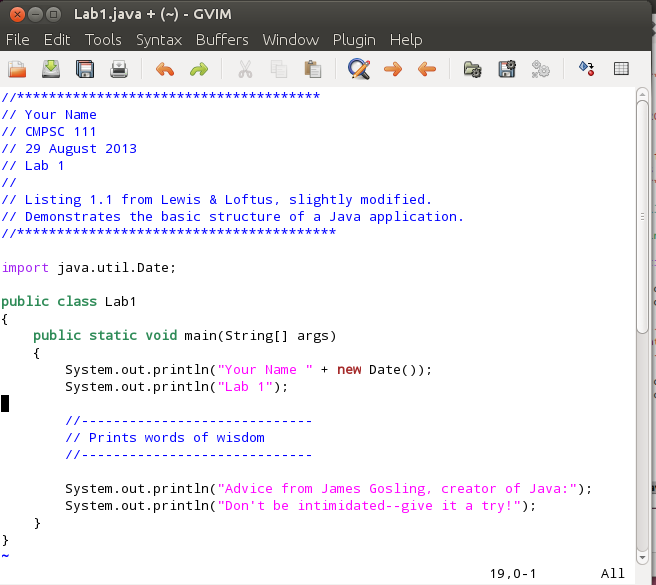
\includegraphics[width=5.8in]{images/lab1prog}
  \caption{Your first program that outputs a quotation from James Gosling.}
  \label{lab1prog}
\end{figure}

Use the ``File/Save'' command to save your program. Alternatively, if you would like to use the keyboard to save your
file, you can press ``:w'' when you are not in insert mode.

       %named ``{\tt cs111/lab1}'' (see Figure \ref{save}).
       %
       %\begin{figure}[htbp]
       %\centering
       %\includegraphics[width=3in]{images/emacssaveas}
       %\caption{Saving the program in the {\tt lab1} folder}
       %\label{save}
       %\end{figure}

Leaving the {\tt gvim} window open, go back to your terminal window. Type the command ``{\tt javac Lab1.java}'' at the
terminal window's prompt---this is the ``compile'' step of writing a Java program that transforms the source code into a
form that can be run on your computer.

% \vspace*{-.1in}
% \begin{quote}
%   \verb$javac Lab1.java$
% \end{quote}
% \vspace*{-.1in}

If you get any error messages, go back into {\tt gvim} and try to figure out what you mis-typed and fix it. Once you
have solved the problem, make a note of the error and the solution for resolving it. Re-save your program and then
re-compile it (i.e., re-run the ``{\tt javac}'' command). If you cannot get the program to compile correctly, then
please talk with the course instructor.

When all errors are eliminated, type ``{\tt java Lab1}'' in the terminal window---this is the ``execute'' step that will
run your program and produce the designated output.  You should see your name, today's date, the lab number, and two
more lines of text. Make sure there are spaces separating words in your output (did you forget to put a space inside the
quotation marks after your last name?). If not, then repair the program and re-compile and re-run it.  Once the program
runs, please reflect on this process.  What step did you find to be the most challenging? Why?

% \begin{quote}
%   \verb$java Lab1$
% \end{quote}


%\begin{figure}[htbp] \centering \includegraphics[width=3.5in]{images/lincolnrun} \caption{Successful compilation and
%execution} \label{output} \end{figure}

Using the ``File/Print'' menu item, print out your program directly from {\tt gvim}. Pick up your output at one of the
two printers in the front of the lab (i.e., 101a or 101b).  Please see the course instructor if you have trouble
printing.  Sign your name at the top of your printout---this is the pledge that the work you are handing in was done
according to the Honor Code guidelines.

       %we'll introduce the
       %``Libre Writer'' application (which you may find useful for other
       %purposes).
       %On the menu on the left, run
       %the ``Libre Writer'' application. Use the ``Insert/File'' menu item to
       %import your {\tt Lincoln.java} program into the document; use the font
       %named ``Courier 10 Pitch'' so that your text appears as fixed-width.
       %
       %Then go back to your terminal window and, with the mouse, highlight
       %everything from the line containing the ``{\tt javac}'' command through
       %the line following your last output line. Copy this (right-click, choose
       %``Copy'') and then paste it at the bottom of your Libre office file.
       %Add a line labeling the program output.
       %
       %The result should look something like Figure \ref{libre}.
       %
       %\begin{figure}[htbp]
       %\centering
       %\includegraphics[width=5.5in]{images/libre}
       %\caption{The Lab Report in Libre Writer}
       %\label{libre}
       %\end{figure}
       %
       %Save your report in your {\tt cs111/lab1} folder with a name like ``{\tt
       %yourname-lab1report.odt}'' (the ``{\tt .odt}'' should be automatically
       %supplied).

       %Now open the Firefox browser and go to {\tt sakai.allegheny.edu}. Log on
       %and go to your ``Drop box''. Under the ``Add'' menu, choose ``Upload Files''.
       %Upload your {\tt Lincoln.java} file {\em AND} your report. (Yes, I want
       %the program uploaded twice, once in the report and once by itself.)
       %{\color{red}\bf[Why?]}

       %Finally, print out your report. You can do this with the ``File/Print''
       %command in Libre Writer.

\vspace*{-.15in}
\subsection*{Write Your Own Program}
\vspace*{-.05in}

Following the steps from the previous part of this laboratory assignment, create a program with a different name (e.g.,
``{\tt Lab1Part2.java}''). Note that the name in your ``{\tt public class}'' statement must exactly match the portion of
the file name preceding the ``{\tt .java}''.  For instance, you must have ``{\tt public class Lab1Part2}'' if the file
name is ``{\tt Lab1Part2.java}''.

Make sure that your program outputs something different than the program that you wrote previously---but still include
your name and the date as shown in the example. Experiment with creating output that includes quotations, art work, or
technical diagrams.  At minimum, this program should create more lines of output than your first one. Try to
purposefully include errors in your program by, for instance, omitting the ``{\tt ;}'', capitalizing something
incorrectly, misspelling a Java keyword, or making other mistakes. As you learn by trying new things, ask additional
questions of or give a status update to the course instructor and a teaching assistant.

Since this is our first laboratory assignment and you are still learning how to use the appropriate hardware and
software, don't become frustrated if you make a mistake. Instead, use your mistakes as an opportunity for learning both
about the necessary technology and the background and expertise of the other students in the class, the teaching
assistants, and the course instructor.

\vspace*{-.1in}
\subsection*{Summary of the Required Deliverables}

This assignment invites you to submit printed and signed versions of the following deliverables:

\vspace*{-.1in}
\begin{enumerate}
  \setlength{\itemsep}{0in}
  \item A commentary on the meaning and purpose of all the commands you typed in the terminal.
  \item A properly commented and formatted version of {\tt Lab1.java} and {\tt Lab1Part2.java}.
  \item The output from running {\tt Lab1} in the terminal window.
  \item The output from running {\tt Lab1Part2} in the terminal window.
\end{enumerate}
\vspace*{-.1in}

In adherence to the Honor Code, students should complete this assignment on an individual basis. While it is appropriate
for students in this class to have high-level conversations about the assignment, it is necessary to distinguish
carefully between the student who discusses the principles underlying a problem with others and the student who produces
assignments that are identical to, or merely variations on, someone else's work.  With the exception of the {\tt
  Lab1.java} program that you created in the first part of the assignment, deliverables that are nearly identical to the
work of others will be taken as evidence of violating the \mbox{Honor Code}.

% \subsection*{Deliverable}
% Hand in your stapled printed programs (there should be at least two, but you might do several more if you want) before
% the due date and time.

\end{document}
